\subsection{Feynman Diagrams} 
Feynman diagrams are a visual way to represent 
our complicated integrals we've defined above. 
We draw Feynman diagrams to 
represent the expansion of $ \bra { f} ( S - 1) \ket{ i } $ and learn to 
associate functions to them (functions of the four momentum). 
We draw an external line for each particle in $ \ket{ i } $
and $ \ket{ f } $, assigning a four dimensional 
4-momentum to each. We add an arrow for  $ \mathbb{C} $  
fields to show flow of charge. 

The first step is to set up our 
initial and final states. 
We choose an in (out) going arrow in $ \ket{ i } $ for a 
particle (antiparticle), and the opposite for final states $ \bra { f} $. 
These are 'external lines' which don't contribute an integral 
since we're just exciting by an operator like $ b_{ \vec{p} } ^ \dagger \ket{ 0 } $. 

\begin{figure}[htpb]
\centering
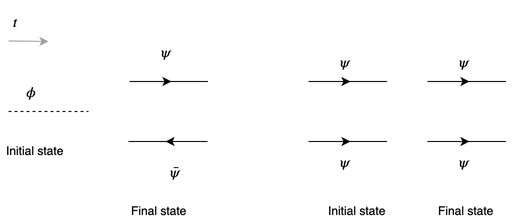
\includegraphics[width=0.8\linewidth]{figures/feyn_1.jpg}
\caption{A template diagram. On the left we have $\phi \to \psi \overline{\psi}$ scattering 
and on the right we have a template for $ \psi \psi \to \psi \psi $ scattering}%
\label{fig:template Feyn}
\end{figure}

We show what kind of diagrams you might have 
for different scattering cases in figure \ref{fig:template Feyn}. 
The next step is to 'fill this in'. We have to be a bit 
careful here. This is is when we need to be aware of what our interaction term looks like. 
For the Yukawa potential, we have our interaction Hamiltonian 
\[
H_I  = \int d^ 3 x \psi ( x) ^ * \psi ( x) \phi ( x) 
\] this means that \textbf{each set of connecting lines} (what we 
call a vertex) in our Feynman diagram needs to look like what we have 
in figure \ref{fig:figures/feyn2}. 
\begin{figure}[htpb]
\centering
\hspace{3cm} \includegraphics[width=0.4\linewidth]{figures/feyn_2.png}
\caption{This is what we must have at each point}%
\label{fig:figures/feyn2}
\end{figure}
We then fill up this diagram with vertices. 
The order of our expansion in $ g $ corresponds 
to how many vertices we have, since each vertex
corresponds to an integral $ \int d^ 4 x H_ I ( x ) $
contributed in Dyson's formula.
Once we've joined together our vertices, we then 
assign a momenta to each line. We have simple examples in the figure. 

\begin{figure}[htpb]
\centering
\includegraphics[width=0.8\linewidth]{figures/feyn_3.png}
\caption{We have some $ O ( g ^ 2 )$ diagrams for $ \psi \psi \to \psi \psi$ scattering}%
\label{fig:figures/feyn_3}
\end{figure}
Our 'internal lines' which are lines with vertices on
both sides are dummy momenta which we integrate over. 
On the other hand, we keep external lines with fixed momenta. 
Each diagram is in 1: 1 correspondence with 
terms in our expansion. 
To each diagram, we evaluate total amplitude using 
Feynman rules for this problem. 
\begin{enumerate}
\item Associate a momentum to each internal line, and keep 
the momenta associated with external legs of the problem 
fixed. 
\item Assign a factor of  $ ( - i g) ( 2 \pi ) ^ 4 \delta ( \sum k_ i ) $
to each vertex, where  $ \sum_i k _ i $ is the sum of 
four momenta flowing \textbf{ in } to the vertex. If momenta 
flows out, this gives a negative momentum contribution. 
\item For each internal line with 4-momenta k, write 
factor 
\[
	\int \frac{ d^ 4 k }{ ( 2 \pi ) ^ 4  } \text{ where } D ( k ^ 2 )  = \begin{cases}
		\frac{ i }{ k ^ 2 - m ^ 2  - i \epsilon } &  \text{ for } \phi \\
		\frac{i }{ k ^ 2 - \mu ^ 2 + i \epsilon } & \text{ for } \psi \\ 
	\end{cases}
\] 
\end{enumerate}
The total amplitude is the sum of all diagrams at the given order. 

